\documentclass{article}
\usepackage[utf8]{inputenc}
\usepackage{amsmath}
\usepackage{amsthm}
\usepackage[left=1in,right=1in,top=1in,bottom=1in]{geometry}
\usepackage{graphicx}
\usepackage{float}
\usepackage{titling}
\usepackage{algorithm}
\usepackage[noend]{algpseudocode}
\usepackage[numbib,nottoc]{tocbibind}
\usepackage{enumitem}
\usepackage{multicol}
\usepackage[numbers]{natbib}
\bibliographystyle{abbrvnat}

\setlist[itemize]{topsep=0pt}
\setlist[enumerate]{topsep=0pt}
\setlength\parindent{0pt}
\setlength{\droptitle}{-1.5cm}

\setlength{\abovedisplayskip}{0pt}
\setlength{\belowdisplayskip}{0pt}
\setlength{\abovedisplayshortskip}{0pt}
\setlength{\belowdisplayshortskip}{0pt}

\newcounter{heuristic} \setcounter{heuristic}{0}
\renewcommand{\theheuristic}{\Alph{heuristic}}

\newenvironment{heuristic}[1]%
{
\refstepcounter{heuristic}
\subsection*{Heuristic \theheuristic: #1}
\vspace{-0.2cm}
}%
{}

\makeatletter
\def\BState{\State\hskip-\ALG@thistlm}
\makeatother

\title{\vspace{-0.8cm}Vertex Coloring and Applications}
\date{May 5, 2017}
\author{\Large{Shawn Seymour\vspace{0.2cm}}\\Directed Study (MATH 3993)\\University of Minnesota Morris}

\makeatletter
\def\thm@space@setup{\thm@preskip=8pt
\thm@postskip=0pt}
\makeatother

\newtheorem{prop}{Proposition}
\newtheorem{theorem}{Theorem}

\theoremstyle{definition}
\newtheorem{definition}{Definition}

\begin{document}

\maketitle

\setlength{\parskip}{0.3cm}

\section{Introduction}
Consider the map of the 48 contiguous states in the USA. Suppose we would like to color each state such that no two states that share a boundary have the same color. How many colors would it take to do this? This problem can be modeled as a \emph{graph}. In general, we could represent every state with a \emph{vertex} and draw an \emph{edge} between two states that share a border. A graph, denoted $G = (V, E)$, is a set of vertices $V$ and a set of edges $E$. A \emph{simple graph} is a loopless, undirected graph where no two edges connect the same pair of vertices. For our purpose, assume all graphs are simple graphs. This problem, along with many others, can be solved using vertex coloring. We can model the map of the 48 contiguous states as a graph. We can represent every state with a vertex and draw an edge between two states that share a border.

\begin{figure}[H]
\centering
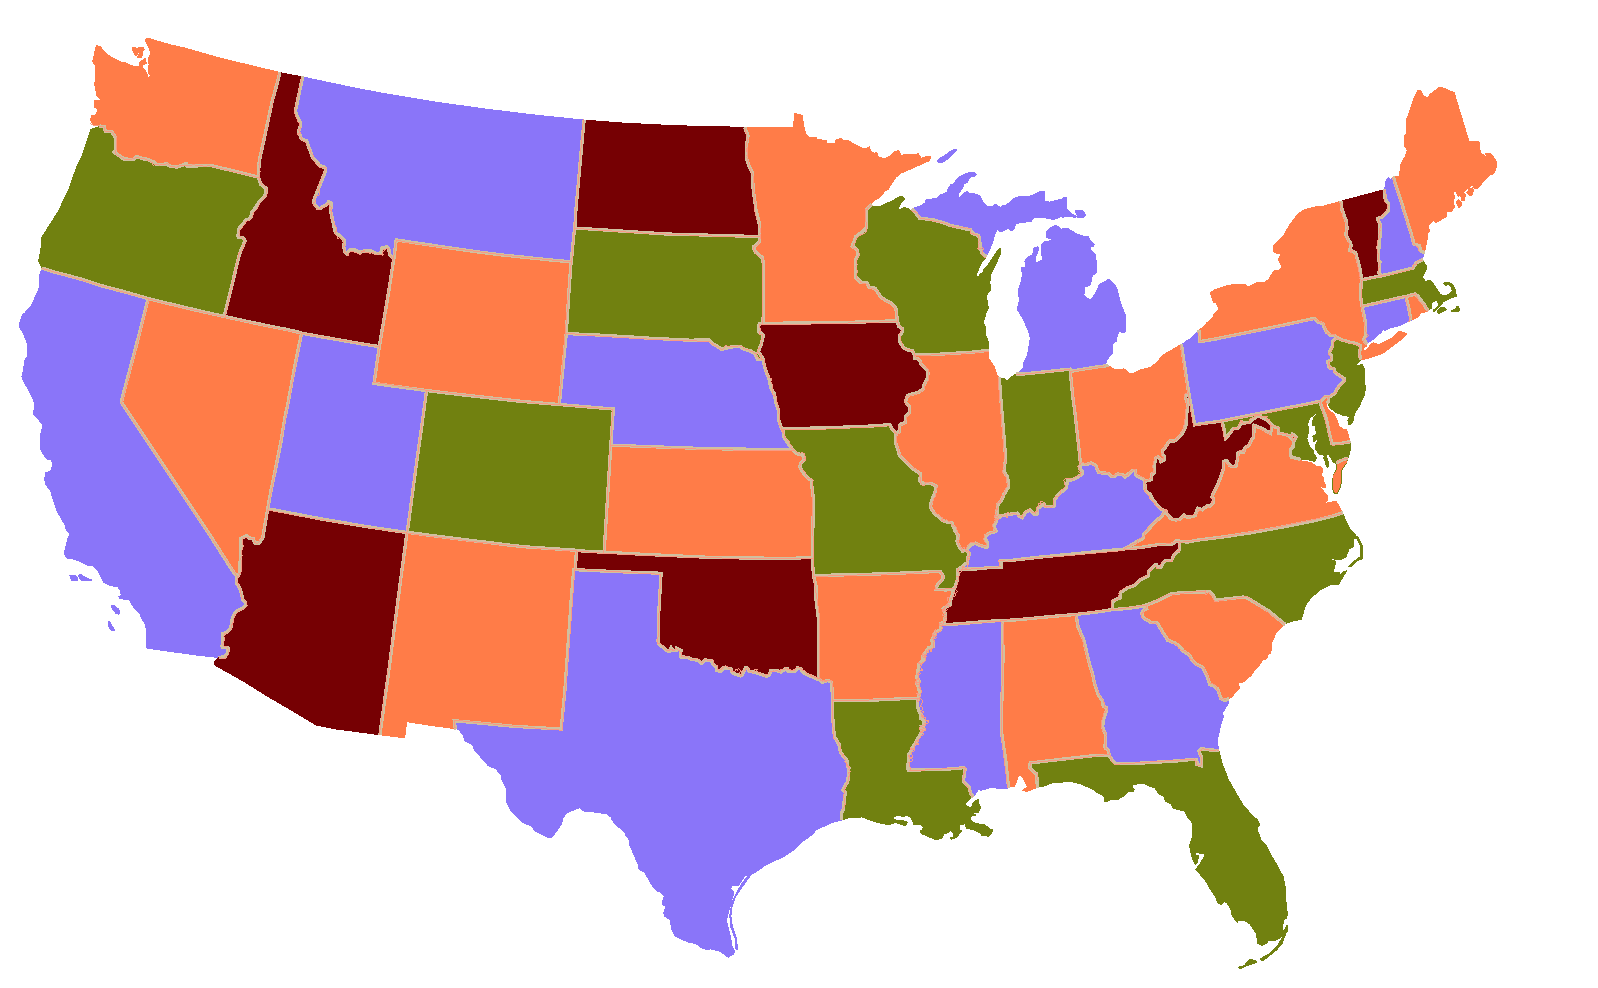
\includegraphics[width=0.7\linewidth]{figures/map-colors.pdf}
\caption{A proper vertex coloring of the 48 contiguous states of the USA}\label{fig:map}
\end{figure}

A \emph{vertex coloring} of a graph $G$ is an assignment of colors to each vertex of a graph. A \emph{proper vertex coloring} assigns colors to a graph $G$ such that no two adjacent vertices share the same color. This can be described as a function $f : V \rightarrow S = \{1, 2, \ldots, k\}$ such that $\forall u,w \in V$, if $(u,w) \in E$, then $f(u) \neq f(w)$. Note that this constraint is the same constraint we applied to our map example. This means we could color our map according to our constraint with a proper vertex coloring. For our purpose, assume we mean proper vertex coloring when referring coloring a graph.

The \emph{chromatic number}, denoted $\chi(G)$, is the minimum number of colors needed to have a proper vertex coloring of a graph $G$. The \emph{vertex coloring problem} (VCP) is to find $\chi(G)$ of any given graph $G$. By applying the vertex coloring problem to our map example, we can determine how many colors one would need to color it with regards to our constraint. An example coloring of our map is shown in Figure \ref{fig:map}. The \emph{k-Colorability problem} asks if a graph can be colored with $k$ colors. If a graph can be colored with $k$ colors, it is said to be \emph{k-colorable}.

\section{Computational Complexity}\label{sec:complexity}
Finding an optimal solution to the vertex coloring problem is not easy. As the VCP is an optimization problem with regards to a constraint, we know it will require heavy computation to find an optimal solution. In mathematics and computer science, we classify computationally complex problems based on type of problem they are and based on how many steps it takes to solve the problem with respect to its input size.

In this section, we will first discuss how to classify hard mathematical problems. Then, we will classify the VCP as a mathematically hard problem and show how this classification can be done.

\subsection{Classifying the Vertex Coloring Problem}
We call any problem that can be answered with ``yes'' or ``no'' a \emph{decision problem}. To classify the vertex coloring problem, we must first introduce some classes, defined by \citet{moret}:

\begin{itemize}
  \item \textbf{P}: Given a decision problem, we can solve the problem in polynomial time.
  \item \textbf{NP}: Given a decision problem, we can verify if a given solution is correct in polynomial time but cannot solve the problem in polynomial time.
  \item \textbf{NP-hard}: Given any problem, it is at least as hard as NP problems. They do not have to be in NP, however, as they do not need to have solutions verifiable in polynomial time.
  \item \textbf{NP-complete}: Given a decision problem, we can transform it to any other NP problem in polynomial time and still verify a given solution in polynomial time.
\end{itemize}

Take note that these classes are not exclusive: any member of P is also a member of NP. NP-complete problems can be thought of as the problems that are both in NP and NP-hard. Although it may seem like all problems that are NP are also NP-complete, this is not the case. There are a select few problems in NP that are not NP-complete or in P. See \citet{ladner1975structure}.

\begin{prop}
The vertex coloring problem is an NP-hard problem.
\end{prop}

It is NP-hard to compute the chromatic number of a graph. This can be proven by showing it is at least as hard as a problem in NP. This is typically done by a reduction (a transformation) to or from 3-SAT, which we'll examine later. This was proven by \citet{garey}.

\begin{prop}\label{prop:k-color-np-complete}
The k-Colorability problem, i.e. can a given graph be colored in k-colors, is NP-complete.
\end{prop}

To prove this, we need to reduce a known NP-complete problem to the vertex coloring problem in polynomial time. By reducing a known NP-complete problem to k-Colorability, we can conclude that k-Colorability is NP-complete as all NP-complete problems are reducible to all other NP-complete problems. See \citet{gareynp}. We will reduce the well-known 3-SAT problem first to the 3-Colorability problem. The 3-Colorability problem asks if a graph can be colored with 3 (or fewer) colors. Obviously, if a graph can be colored with 2 colors it can also be colored with 3.  From here, the reduction from 3-Colorability to k-Colorability follows.

\subsection{Reduction from 3-SAT to 3-Colorability}
Before we prove Proposition \ref{prop:k-color-np-complete}, we must first introduce 3-SAT.  The 3-SAT problem is a decision problem that is a variation of the original NP-complete problem, Boolean satisfiability (SAT). The 3-SAT problem was proven to be NP-complete. See \citet{gareynp}. SAT consists of a conjunction of $m$ clauses, i.e. $C_1 \wedge C_2 \wedge \dots \wedge C_m$. Each clause is a disjunction of at most $n$ literals, i.e. $L_1 \vee L_2 \vee \dots \vee L_n$. Each literal can be a variable or negative of a variable, i.e. $x_1, \neg x_1, x_2, \neg x_2, \dots , x_k, \neg x_k$ where $k$ is the number of distinct literals. Each literal has a value of $true$ or $false$. 3-SAT has exactly 3 literals in each clause $(n = 3)$. We will assume all of our satisfiability problems are in conjunctive normal form (CNF). 3-SAT asks whether the variables can be assigned \emph{true} or \emph{false} in such a way that the whole expression evaluates to \emph{true}. We define SAT and 3-SAT in Definition \ref{def:sat}.

\begin{definition}\label{def:sat}
SAT is a decision problem that decides the truth value of a Boolean function based on the evaluation of the clause. It determines whether there are truth values to each clause in a set of clauses that will return a truth value to the given Boolean function. 3-SAT is a variation of SAT where each clause contains exactly 3 literals.
\end{definition}

To show a reduction from 3-SAT to 3-Colorability, we need to:

\begin{enumerate}
\item Construct an instance of 3-Colorability, given an instance of 3-SAT
\item Show that if the resulting graph is 3-colorable, then the given 3-SAT problem is satisfied
\end{enumerate}

To show this reduction, we'll create an example 3-SAT problem and reduce it to 3-Colorability. This reduction will create a graph \(G = (V, E)\) having \((2n + 3m + 1)\) vertices and \((3n+6m)\) edges. See \citet{moret}. The process for creating the graph, described below, was taken from the proof given by \citet{sharma}.

Let's introduce the following 3-SAT expression $E$:
%
\begin{align*}
E = \left( x_1 \vee \neg x_2 \vee \neg x_3 \right) \wedge \left( \neg x_1 \vee x_2 \vee x_3 \right) \wedge \left( x_1 \vee x_2 \vee x_3 \right)
\end{align*}
%
To create the graph of this 3-SAT problem, we:
\begin{enumerate}
\item Create a \emph{triangle} for each variable, i.e. \(x_i\). Each has a common vertex \(B\), called the base vertex. This base vertex will be colored a color, say \(p_1\), so that the other two vertices correspond to the variable and it's negation.
\item Create a \emph{triangle} for each clause in the formula.
\item Connect each vertex of a clause triangle to the corresponding literal vertex.
\end{enumerate}

Following the above steps, we generate graph $G$, shown in Figure \ref{fig:3sat1}, from our 3-SAT expression $E$.

\begin{figure}[H]
\centering
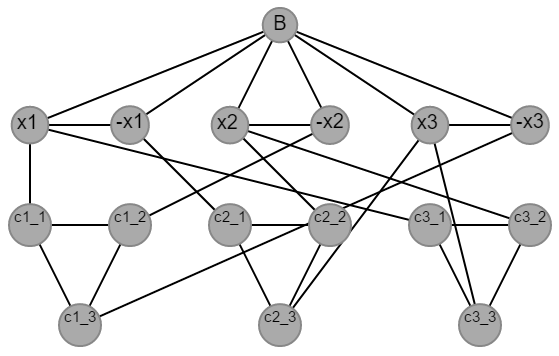
\includegraphics[scale=0.6]{images/3sat-1.png}
\caption{\(E\) represented as a graph \(G\)}\label{fig:3sat1}
\end{figure}

If we can properly color graph \(G\) with 3 colors, then the original 3-SAT is satisfiable and the truth values of the variables are denoted by the color they received. This graph is \emph{3-colorable} and the coloring is shown in Figure \ref{fig:3sat2}.

\begin{figure}[H]
\centering
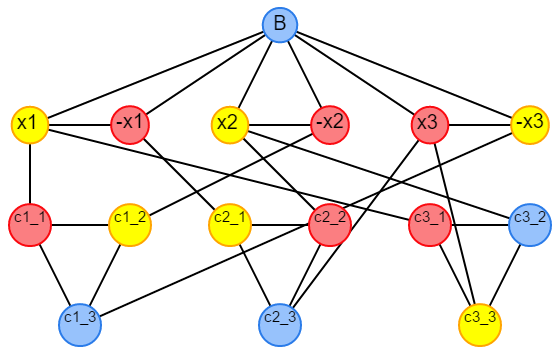
\includegraphics[scale=0.6]{images/3sat-2.png}
\caption{A possible 3-coloring of \(G\)}\label{fig:3sat2}
\end{figure}

As we see above, \emph{blue} is used for the base vertex and as part of some of the clause triangles. If we let \emph{yellow} denote \emph{true} and \emph{red} denote \emph{false}, we can see that our original 3-SAT is satisfied:
%
\begin{align*}
E &= \left( T \vee \neg T \vee \neg F \right) \wedge \left( \neg T \vee T \vee F \right) \wedge \left(T \vee T \vee F \right) \\
&= \left( T \vee F \vee T \right) \wedge \left( F \vee T \vee F \right) \wedge \left(T \vee T \vee F \right) \\
&= T \wedge T \wedge T \\
&= True
\end{align*}
%
This shows an example of the reduction from 3-SAT to 3-Colorability. If \(G\) was unable to be colored with 3 colors, then we would know that \(E\) is unable to be satisfied. From here, we can reduce 3-Colorability to 4-Colorability, and then generalize that reduction and reduce 4-Colorability to k-Colorability. The proof and illustration of this can be found in \citet{sharma}.

\section{Heuristics}
As we have seen in section \ref{sec:complexity}, the vertex coloring problem is NP-hard and thus solving it to optimality for any given instance of a graph is computationally ``impossible''. This gives us incentive to use approximation algorithms, called heuristics, to find good, but not necessarily optimal, vertex colorings. We will analyze and compare a few of the popular heuristics for solving the VCP. However, in this section, we will describe the four heuristics to solve the VCP. The input for all heuristics we define is a simple graph, $G = (V, E)$.

\newpage

\heuristic{Greedy}\label{heuristic-greedy}

Heuristic \ref{heuristic-greedy} is a simple greedy algorithm. It is defined in Algorithm \ref{alg:greedy}.

\begin{algorithm}
\caption{Greedy algorithm}\label{alg:greedy}
\begin{algorithmic}[1]
\State Label each vertex in $V$, i.e. $v_1, v_2, \dots, v_n$
\For{each $v \in V$}
\State Assign a color $p_i$ to $v_i$ using the smallest available $p_i$
\EndFor
\end{algorithmic}
\end{algorithm}

\heuristic{Welsh-Powell}\label{heuristic-welsh}

Heuristic \ref{heuristic-welsh} is the greedy algorithm with degree sequencing. Before applying the greedy algorithm, it orders the vertices according to the decreasing value of their degree. This is also known as the Welsh-Powell algorithm, which was defined by \citet{welsh}. It is defined in Algorithm \ref{alg:welsh}.

\begin{algorithm}
\caption{Welsh-Powell algorithm}\label{alg:welsh}
\begin{algorithmic}[1]
\State Label each vertex in $V$, i.e. $v_1, v_2, \dots, v_n$, such that $d_G(v_1) \geq d_G(v_2) \geq \dots \geq d_G(v_n)$
\ForAll{$v \in V$}
\State Assign a color $p_i$ to $v_i$ using the smallest available $p_i$
\EndFor
\end{algorithmic}
\end{algorithm}

\heuristic{DSATUR}\label{heuristic-dsatur}

Heuristic \ref{heuristic-dsatur} is very similar to heuristic \ref{heuristic-welsh}, but colors a graoh based on the \emph{saturation} degree of vertices, which is defined in Definition \ref{def:saturation} \cite{spinrad}. The original DSATUR algorithm was proposed by \citet{brelaz}. It is defined in Algorithm \ref{alg:dsatur}.

\begin{definition}[Saturation degree]\label{def:saturation}
The saturation degree of a vertex is the number of different colors used for vertices adjacency to it.
\end{definition}

\begin{algorithm}
\caption{DSATUR algorithm}\label{alg:dsatur}
\begin{algorithmic}[1]
\State Find the vertex $\in V$ with maximum degree and color it with color $p_1$
\While{There are uncolored vertices}
\State Choose an uncolored vertex with maximum saturation degree
\State If there is a tie, choose the vertex with maximum degree
\State Color the vertex with the least possible number
\EndWhile
\end{algorithmic}
\end{algorithm}

\heuristic{Maximal Independent Set}\label{heuristic-mis}

Heuristic \ref{heuristic-mis} colors a graph by finding maximal independent sets of \(G\). A maximal independent set (MIS) is defined in Definition \ref{def:mis}. This is quite different than our other heuristics as it does not depend on degree. Ideally, we would want to find a maximum independent set, not just a maximal independent set.

Finding a maximum independent set is NP-hard as detailed by \citet{karp1972reducibility}. This means we're including a different NP-hard in an already NP-hard problem. We chose to forgo this in favor of just finding a maximal independent set. We define the heuristic in Algorithm \ref{alg:mis}.

\begin{definition}[Maximal independent set]\label{def:mis}
An independent set is a subset $S$ of vertices in a graph such that no two vertices in the set are adjacent. $S$ is said to be maximal if no vertex outside the set can be added while still being an independent set.
\end{definition}

\begin{algorithm}
\caption{Maximal independent set algorithm}\label{alg:mis}
\begin{algorithmic}[1]
\State $p \leftarrow 1$
\While{$G$ is non-empty}
\State Find a maximal independent set of $G$, i.e. $S_i$
\State Color all vertices in $S_i$ with color $p$
\State Let $G \leftarrow G[V \setminus S_i ] $
\State $p \leftarrow p + 1$
\EndWhile
\end{algorithmic}
\end{algorithm}

\section{Analysis of Heuristics A - D}
Before comparing the heuristics, we first wanted to analyze the heuristics individually and look at the solutions they produce.

\begin{prop}
Heuristic \ref{heuristic-greedy} and Heuristic \ref{heuristic-welsh} produce a feasible, proper coloring of input graph \(G = (V, E)\).
\end{prop}

Let \(G = (V, E)\) be a simple graph. Assume that two vertices, say \(v_1, v_2 \in V\), are connected by an edge \(e_1 \in E\). Assume that \(v_1, v_2\) are colored the same color, say \(p_1\). We know that in both heuristics, we assign the smallest color \(p_i\) that is not being used by any of the neighboring vertices connected by an edge \(e_i\). WLOG, the heuristic would color \(v_1\) color \(p_1\). The next iteration, while vertex \(v_2\) is selected, the heuristic would see color \(p_1\) is assigned to a neighboring vertex \((v_1)\), and assign the next available color \(p_2\). Thus, we've reached a contradiction.

\begin{prop}
Heuristic \ref{heuristic-dsatur} produces a feasible, proper coloring of input graph \(G = (V, E)\).
\end{prop}

Let \(G = (V, E)\) be a simple graph. We color the vertex with the maximum degree color 1. If there are no uncolored vertices, we have properly colored $G$. If there are, then we find an uncolored vertex $v$ with maximum saturation degree. We then color $v$ with the smallest available color. This means we look at the set of all adjacent vertices to $v$ and find the smallest unused color in this set. This means we will never color an adjacent vertex with the same color, and thus, will always result in a proper coloring.

\begin{prop}
Heuristic \ref{heuristic-mis} produces a feasible, proper coloring of input graph \(G = (V, E)\).
\end{prop}

Let \(G = (V, E)\) be a simple graph. Let $p$, the current color, be 1. By definition \ref{def:mis}, we know that no two vertices in a maximal independent set are adjacent. Thus, when we color the vertices in the MIS with the smallest color \(p_1\) for the first iteration, we know that it is properly colored. We then remove the found maximal independent set and increment $p$ to 2. If $G$ is now empty, then $G$ is properly colored. If $G$ is not empty, then we repeat the process except we use color 2. Because we are always incrementing the color for each iteration, we know the MIS found will always be properly colored with a different color than the past MIS.

Now that we know our heuristics produce feasible, proper colorings of a graph, how do we know they do not produce optimal solutions? We show they do not using counterexamples.

\begin{prop}
Heuristic \ref{heuristic-greedy} and Heuristic \ref{heuristic-welsh} do not produce optimal solutions, i.e. they do not always produce a minimum coloring for all graphs.
\end{prop}

We will show this for \emph{heuristic \ref{heuristic-welsh}}. It is trivial to show the same for \emph{heuristic \ref{heuristic-greedy}} as \emph{heuristic \ref{heuristic-welsh}} includes the same steps as \emph{heuristic \ref{heuristic-greedy}}. We will construct a simple graph, \(G = (V, E)\), such that:
%
\begin{align}
|V| &\geq 8 \\
\chi(G) &> \chi^{*}(G)
\end{align}
%
Let \(\chi(G)\) refer to the coloring of \(G\) generated by \emph{heuristic \ref{heuristic-welsh}}. Let \(\chi^{*}(G)\) be the optimal coloring of \(G\). We constructed a simple graph, \(G_1 = (V, E)\), such that \(\Delta(G_1) = 3\) and \(\delta(G_1) = 1\).

\begin{figure}[H]
\centering
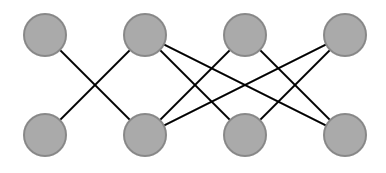
\includegraphics[scale=0.5]{images/graph-1.png}
\caption{Uncolored original graph \(G_1\)}
\end{figure}

By applying \emph{heuristic \ref{heuristic-welsh}}, we get the following coloring. The numbers indicate the order the vertices were colored in while applying the heuristic. Any vertex of the same degree got assigned arbitrarily. This results in \(\chi(G_1) = 3\).

\begin{multicols}{2}
  \begin{figure}[H]
  \centering
  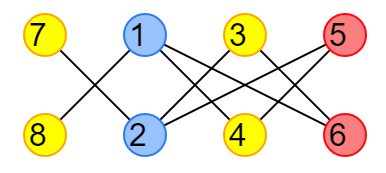
\includegraphics[scale=0.5]{images/graph-2.png}
  \caption{Coloring of $G_1$ after applying heuristic \ref{heuristic-welsh}}
  \end{figure}

  \begin{figure}[H]
  \centering
  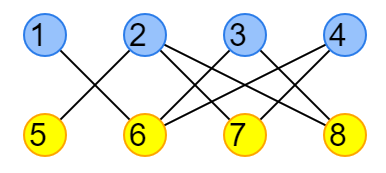
\includegraphics[scale=0.5]{images/graph-3.png}
  \caption{Optimal coloring of graph \(G_1\)}\label{fig:ex1-optimal}
  \end{figure}
\end{multicols}

\begin{definition}[Bipartite graph]
A bipartite graph is one whose vertex set can be partitioned into two subsets X and Y such that each edge has one end in X and one end in Y.
\end{definition}

We can see that $G_1$ is a bipartite graph. Thus, \(G_1\) is 2-colorable as all bipartite graphs are 2-colorable. See \citet{asratian1998bipartite}. This means \(\chi^{*}(G_1) = 2\). \(G_1\) is an example graph that satisfies our given conditions \((1)\) and \((2)\). The optimal coloring is shown in Figure \ref{fig:ex1-optimal}.



Although Heuristic \ref{heuristic-greedy} and Heuristic \ref{heuristic-welsh} do not always produce an optimal coloring for bipartite graphs, Heuristic \ref{heuristic-dsatur} always will produce an optimal coloring (2 colors). Heuristic \ref{heuristic-dsatur}, however, does not produce optimal colorings for all graphs. Both of these results are shown and proven by \citet{brelaz}.

\begin{prop}
Heuristic \ref{heuristic-dsatur} does not produce an optimal solution, i.e. it does not always produce a minimum coloring for all graphs.
\end{prop}

To show this, we've created a graph $G_2 = (V, E)$ for this example. This is shown in.

\begin{figure}[H]
\centering
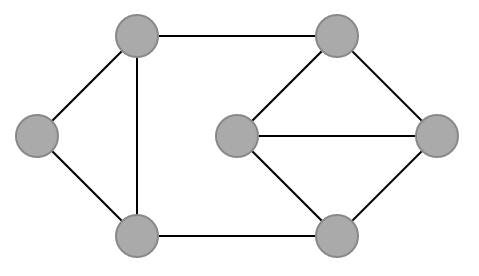
\includegraphics[scale=0.5]{images/dsatur-1.png}
\caption{Uncolored original graph \(G_2\)}\label{fig:ex2-uncolored}
\end{figure}

By applying heuristic \ref{heuristic-dsatur}, we can see that $G_2$ is \emph{4-colorable}. This is shown in Figure \ref{fig:ex2-colored}.

\begin{multicols}{2}
  \begin{figure}[H]
  \centering
  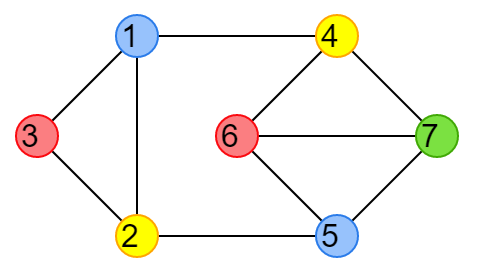
\includegraphics[scale=0.5]{images/dsatur-2.png}
  \caption{Coloring of \(G_2\) after applying heuristic \ref{heuristic-dsatur}}\label{fig:ex2-colored}
  \end{figure}

  \begin{figure}[H]
  \centering
  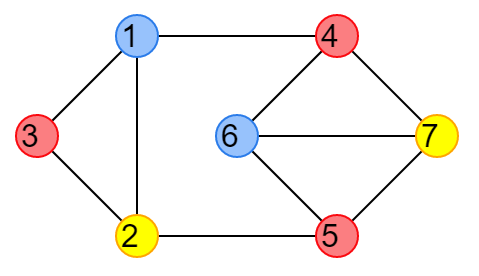
\includegraphics[scale=0.5]{images/dsatur-3.png}
  \caption{Optimal coloring of \(G_2\)}\label{fig:ex2-optimal}
  \end{figure}
\end{multicols}

This is a non-optimal solution as this graph is \emph{3-colorable}. This means \(\chi^{*}(G_2) = 3\). Thus, we can see that heuristic \ref{heuristic-dsatur} does not always give us an optimal solution. The optimal coloring of $G_2$ is shown in Figure \ref{fig:ex2-optimal}.

\begin{prop}
Heuristic \ref{heuristic-mis} does not produce an optimal solution, i.e. it does not always produce a minimum coloring for all graphs.
\end{prop}

To show this, we will create another example that satisfies conditions \((1)\) and \((2)\) from earlier. We've constructed a graph \(G_3 = (V,E)\) for this example. This is shown Figure \ref{fig:ex3-uncolored}.

\begin{figure}[H]
\centering
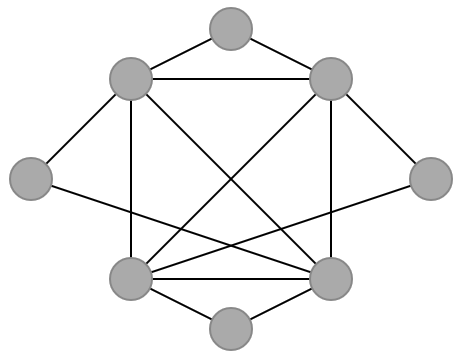
\includegraphics[scale=0.5]{images/mis-1.png}
\caption{Uncolored original graph \(G_3\)}\label{fig:ex3-uncolored}
\end{figure}

By applying heuristic \ref{heuristic-mis} and finding maximal independent sets, we see that \(G_3\) is \emph{5-colorable}. This is shown Figure \ref{fig:ex3-colored}.

\newpage

\begin{multicols}{2}
  \begin{figure}[H]
  \centering
  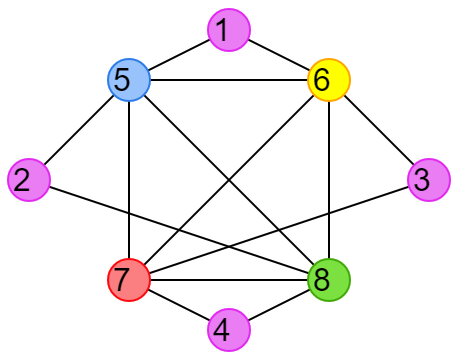
\includegraphics[scale=0.5]{images/mis-2.png}
  \caption{Coloring of \(G_3\) after applying heuristic \ref{heuristic-mis}}\label{fig:ex3-colored}
  \end{figure}

  \begin{figure}[H]
  \centering
  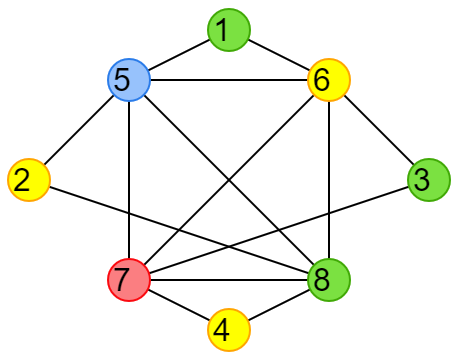
\includegraphics[scale=0.5]{images/mis-3.png}
  \caption{Optimal coloring of \(G_3\)}\label{fig:ex3-optimal}
  \end{figure}
\end{multicols}

This is a non-optimal solution. We can see that the subgraph created by vertices \(\{5, 6, 7, 8\}\) is complete and thus we need at least 4 colors. This graph is \emph{4-colorable} however, meaning \(\chi^{*}(G_3) = 4\). Thus, we can see that heuristic \ref{heuristic-mis} does not always give us an optimal solution. The optimal coloring of $G_3$ is shown in Figure \ref{fig:ex3-optimal}.

\begin{prop}
Heuristic \ref{heuristic-greedy} and heuristic \ref{heuristic-welsh} yield an upper bound of \(\Delta + 1\).
\end{prop}

To show this, we will create another example that satisfies conditions \((1)\) and \((2)\) from above. After doing some research into bipartite graphs, we learned that \emph{crown graphs} are excellent at showing how bad greedy heuristics can be, as shown and defined by \citet{kordecki}.

\begin{definition}[Crown Graph]
A crown graph \(CR_n = (V, E)\) is an undirected graph such that \(U = \{u_1, u_2, \dots, u_i\}\) and \(W = \{w_1, w_2, \dots, w_j\}\) where \(V = U \cup W\), \(U \cap W = \emptyset\), and \(|U| = |W|\). There is an edge from \(u_i\) to \(w_j\) whenever \(i \neq j\). A crown graph can also be viewed as a complete bipartite graph where the edges of a perfect matching have been removed.
\end{definition}

We constructed a simple crown graph, \(G_3 = (V, E)\). We've let \(|V| = 10\) for this example.


\begin{figure}[H]
\centering
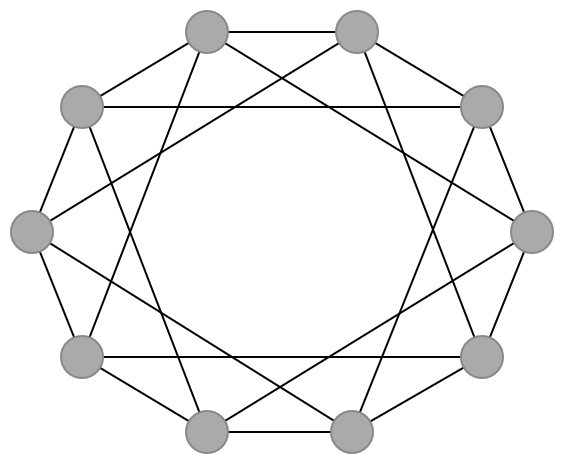
\includegraphics[scale=0.38]{images/graph-4.png}
\caption{Uncolored original graph \(G_4\)}
\end{figure}

We can see that \(\Delta(G_4) = 4\). We can also see \(d_{G_4}(v) = 4\) for all \(v \in V\). Thus, in both heuristics \ref{heuristic-greedy} and \ref{heuristic-welsh}, the algorithm would pick an order arbitrarily. We can show using this crown graph the worst-case scenario of these heuristics.

\begin{multicols}{2}
  \begin{figure}[H]
  \centering
  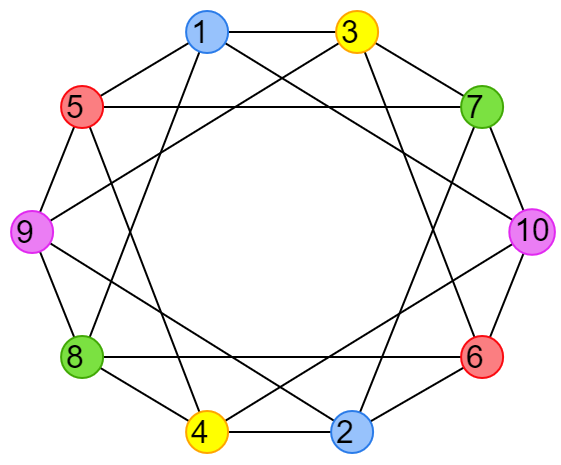
\includegraphics[scale=0.38]{images/graph-5.png}
  \caption{Worst-case coloring of \(G_4\)}\label{fig:ex4-colored}
  \end{figure}

  \begin{figure}[H]
  \centering
  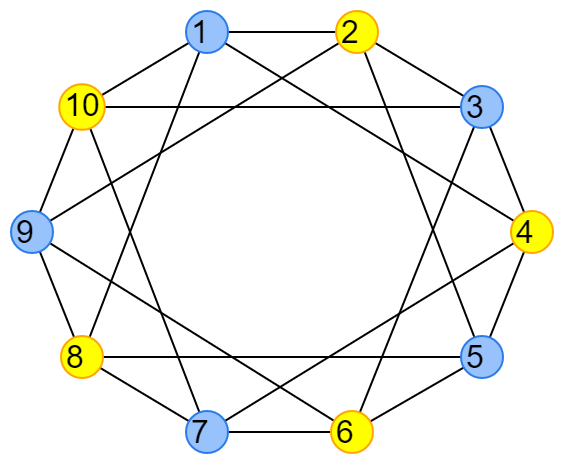
\includegraphics[scale=0.38]{images/graph-6.png}
  \caption{Optimal coloring of \(G_4\)}\label{fig:ex4-optimal}
  \end{figure}
\end{multicols}

\vspace{-0.3cm}

As shown in Figure \ref{fig:ex4-colored}, using either heuristic with this ordering, we get \(\chi(G_4) = 5\). This gives us \(\frac{|V|}{2}\) colors. This is the worst-case for a crown graph. See \citet{johnson}. This graph also demonstrates the upper bounds for these heuristics.

Let's take a look at how this looks in general. Let \(P = (V, E)\) be a simple, complete graph. We can see that \(\chi(H) = \Delta(H) + 1\). This is very easy to see in a \emph{complete} graph, where all vertices are connected to every other vertex. This means all vertices have degree \(|V| - 1\). Thus, every time we color a node, a new color is needed. And since we have \(\Delta(P) = |V| - 1\) and \(|V|\) vertices, we will need \(\Delta(P) + 1\) colors. This is stated in \emph{Brooks' Theorem}.

\begin{theorem}[Brooks' Theorem]
For any connected undirected graph \(G\) with maximum degree \(\Delta\), the chromatic number of \(G\) is at most \(\Delta\) unless \(G\) is a complete graph or an odd cycle, in which case the chromatic number is \(\Delta + 1\).
\end{theorem}

The proof of Brook's Theorem is shown by \citet{lovasz}. Overall, heuristics can produce undesirable results compared to the optimal solution. In graph \(G_4\), in the worst case, some heuristics produce \(\chi(G_4) = 5\) when \(\chi^{*}(G_4) = 2\) as it is a bipartite graph. This is shown in Figure \ref{fig:ex4-optimal}.

\vspace{-0.1cm}

\section{Results}
Our main goal was to compare these heuristics to find out which heuristic was most effective in efficiently approximating the vertex coloring problem. we wanted to compare both quality (number of colors used) and efficiency (running time). For this study, we decided to omit the maximal independent set heuristic (heuristic \ref{heuristic-mis}) as it was so different from the other 3 as well as including another NP-hard problem. We implemented the three heuristics in Java and ran simulations according to the following:
\begin{itemize}
  \setlength\itemsep{0.4em}
  \item Graphs were randomly generated based on the \emph{Erdős–Rényi} model, given in \citet{erdds1959random}. This model generates a random graph with approximately $p$ percent of edges.
  \item We analyzed graphs with $10\%, 20\%, \ldots, 90\%$ edges. We called this the type of the graph. This gave us both sparse and dense graphs.
  \item Simulations were run on graphs with 5 different amount of vertices: 50, 100, 250, 500, 1000.
\end{itemize}

We used statistical analysis to compare the number of colors used and the running time of each heuristic based on edge percentage (type) and then also looked at how this changed as the number of vertices changed.

\begin{figure}[H]
  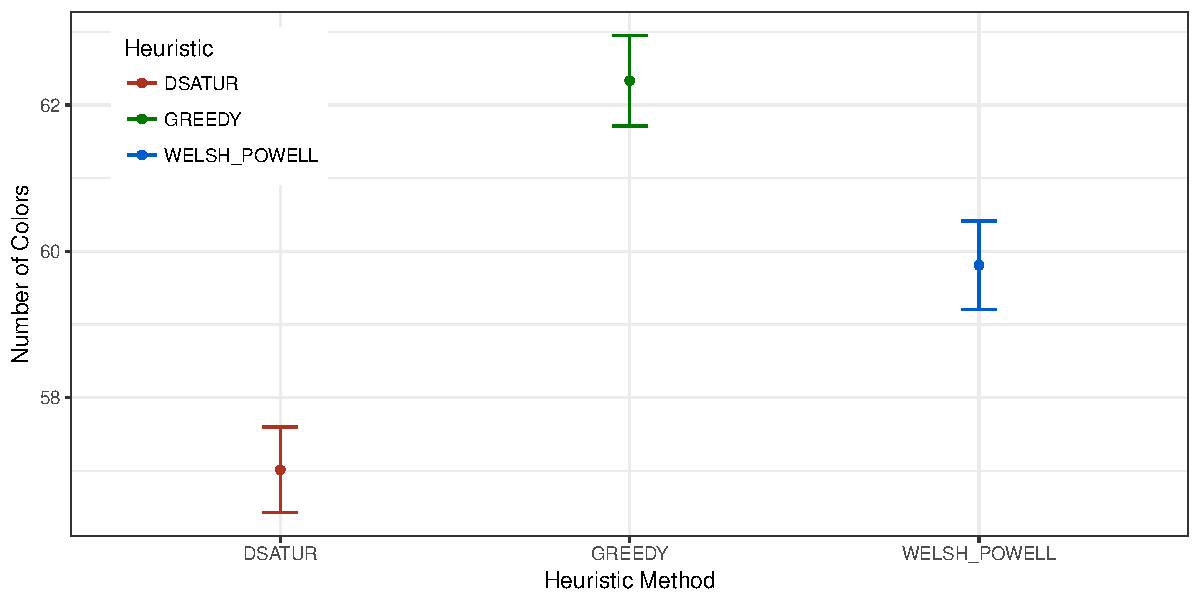
\includegraphics[width=\linewidth]{../poster/figures/plot-colors.pdf}
  \caption{Number of colors used for the three heuristics of graphs with 50, 100, 250, 500, \& 1000 vertices}\label{fig:compare-colors}
\end{figure}

Based on computational data of the amount of colors used, as shown in Figure \ref{fig:compare-colors}, we found:
\begin{itemize}
  \item Heuristic \ref{heuristic-greedy} (Greedy) uses on average 2.52 colors more than Heuristic \ref{heuristic-welsh} (Welsh-Powell).
  \item Heuristic \ref{heuristic-welsh} (Welsh-Powell) uses on average 2.79 colors more than Heuristic \ref{heuristic-dsatur} (DSATUR).
\end{itemize}
This led us to the following partial order based on colors used, where $X \preceq Y$ means heuristic $X$ uses significantly more colors than heuristic $Y$.
\begin{center}
  \textbf{Greedy $\preceq$ Welsh-Powell $\preceq$ DSATUR}
\end{center}
As vertices increased, the partial order defined above stays consistent. Heuristic \ref{heuristic-dsatur} (DSATUR) always used the least colors while Heuristic \ref{heuristic-greedy} (Greedy) always used the most.

Based on computational data of the running time, as shown in Figure \ref{fig:compare-time}, we found:
\begin{itemize}
  \item Welsh-Powell is significantly slower than Greedy.
  \item DSATUR is significantly slower than Welsh-Powell.
\end{itemize}
This led us to the following partial order based on running time, where $X \preceq Y$ means heuristic $X$ uses significantly less time than heuristic $Y$.
\begin{center}
  \textbf{Greedy $\preceq$ Welsh-Powell $\preceq$ DSATUR}
\end{center}

\newpage

As the edge percentage increases:
\begin{itemize}
  \item Heuristic \ref{heuristic-dsatur} (DSATUR) running time increases.
  \item Heuristic \ref{heuristic-greedy} (Greedy) and Heuristic \ref{heuristic-welsh} (Welsh-Powell) running time increases until 50\% edges then decreases until 90\% edges.
  \item The difference in running time between DSATUR and Greedy as well as DSATUR and Welsh-Powell grows larger and larger.
\end{itemize}

\begin{figure}[H]
  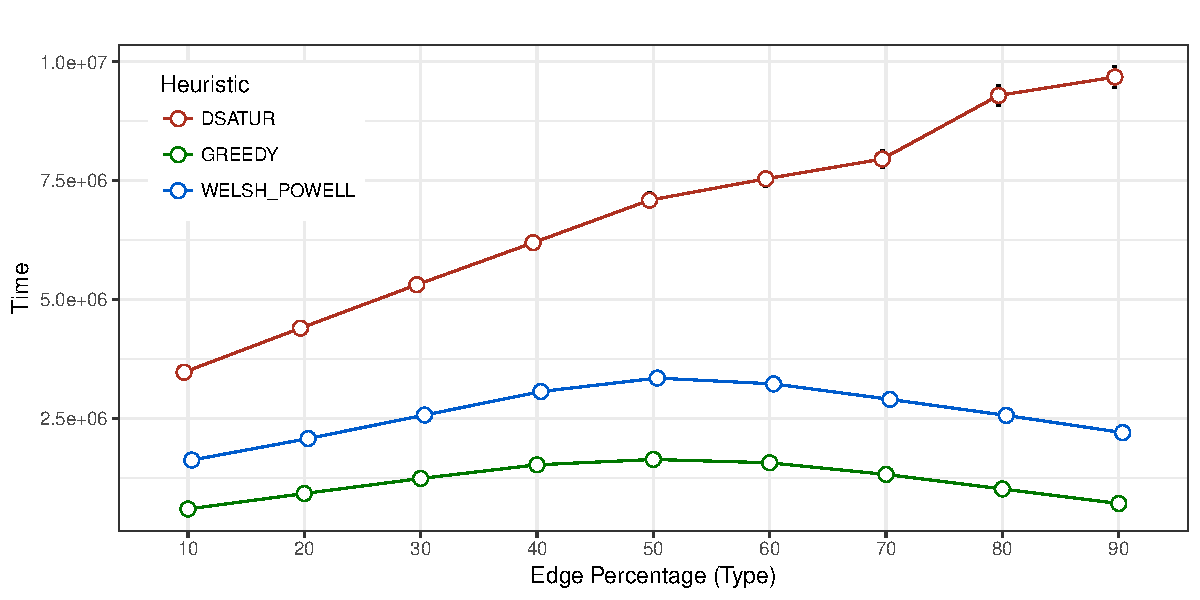
\includegraphics[width=\linewidth]{../poster/figures/plot-time.pdf}
  \caption{Running time for each edge percentage of graphs with 50, 100, 250, 500, \& 1000 vertices}\label{fig:compare-time}
\end{figure}

\section{Conclusion}
Although we were not able to compare the coloring of the heuristics to the optimal coloring, we were able to determine which heuristics gave the closest to the optimal solution. We found that Heuristic \ref{heuristic-dsatur} (DSATUR) produced the lowest number of colors. However, DSATUR also utilized the most time especially as the edge percentage of the graph grew. This is undesirable, because in large graphs, this defeats our purpose of using heuristics to efficiently approximate the VCP.

Based on our overall results, we would suggest using Heuristic \ref{heuristic-welsh} (Welsh-Powell) for most graphs. This is because the extra time needed from Heuristic \ref{heuristic-greedy} (Greedy) to Heuristic \ref{heuristic-welsh} (Welsh-Powell) to achieve better accuracy is not as significant compared to the extra time needed from Heuristic \ref{heuristic-welsh} (Welsh-Powell) to  Heuristic \ref{heuristic-dsatur} (DSATUR).



\newpage

\bibliography{references}

\end{document}
